\chapter{Vórtices ópticos}
\label{cap:vortices}

Una singularidad es una indeterminación en un campo, por lo que tanto la fase como la amplitud son nulas; y puede presentarse en diversos sistemas físicos. En el caso de la óptica, los haces que poseen esta características se conocen con el nombre de vórtices ópticos (OVs: \textit{optical vortices}).\\

A lo largo de este capítulo abarcaremos de manera introductoria el concepto de vórtice óptico y nos centraremos en las diferentes maneras en las cuales éstos pueden producirse. A partir de ello, analizaremos las características de un modulador espacial de luz (SLM: \textit{spatial light modulator}) elemento usado en este proyecto para generar OVs. para finalmente, analizar el efecto de un SLM de transmisión sobre las características de los OVs. Comenzaremos con una revisión del estado del arte de las singularidades en la sección \ref{sec:hist_vor} para proceder con la definición de OV y algunas de sus características en la sección \ref{sec:vortice_optico}. A continuación, en la sección \ref{sec:generacion_vortices} trataremos la generación de OVs partir de elementos de fase. Luego en la Sección \ref{sec:slm} nos centraremos en los SLM. Finalmente en la sección \ref{sec:genvoslm} analizaremos la repercusión de un SLM no ideal en la generación de OVs.

%interpretar algunas de las aberraciones que los OVs poseen brindan información de los elementos del sistema 

%En este primer capítulo trataremos los vórtices ópticos (OVs: \textit{optical vortices}) que han permitido el desarrollo de una rama de la óptica denominada \textit{óptica singular}.
%La importancia de tratar los OVs radica en que este proyecto está basado en la caracterización de aberraciones que éstos presentan, las cuales pueden provenir de diferentes fuentes, tales como el sistema óptico o bien los elementos empleados para la generación de sus características. Es por ello que a lo largo de este capítulo abarcaremos de manera general e introductoria aspectos fundamentales de los OVs para finalmente comprender por qué algunas de las aberraciones que éstos presentan pueden dar información además del sistema óptico, de algunos de los elementos que se emplean en su generación. En adelante, en la sección \ref{sec:hist_vor} se realizará un breve contexto histórico para explicar en la sección \ref{sec:vortice_optico} qué es un OV y su modelación matemática. La sección \ref{sec:generacion_vortices} muestra de qué manera se han obtenido OVs modificando la fase o la amplitud de un plano objeto. En la sección \ref{sec:slm} se profundizará en uno de los elementos más comunes para la generación de OVs, como lo es un modulador espacial de luz (SLM: \textit{spatial light modulator}), con esto se comprenderá qué características mínimas debe cumplir para generar OVs de alta calidad óptica, para finalmente en la sección \ref{sec:genvoslm} analizar los efectos que tiene un SLM de baja calidad sobre los VOs.

\section{Introducción}
\label{sec:hist_vor}

Los sistemas físicos que poseen singularidades han sido estudiados desde la década de 1830, siendo los puntos anfidrómicos\footnote{Punto de amplitud zero en el armónico constituyente de una onda, de forma que la superposición de ondas provenientes de diferentes direcciones causa que un punto posea amplitud cero (que no haya movimiento causado por las ondas en ese punto).} producido por las olas del mar los primeros casos de ello \cite{Berry2000}. En estos puntos debido a la convergencia de olas con diferentes direcciones, la interferencia hace que la amplitud sea nula y las olas parecieran provenir desde él. Este estudio sería luego expandido por Whewell \cite{Whewell1830}, observando diferentes puntos anfidrómicos ubicados en el Mar del Norte en Europa y posteriormente en toda la superficie marina. En la misma década, durante la postulación de los monopolos magnéticos en la teoría cuántica, Dirac \cite{Dirac1931} apreció la existencia de singularidades en la fase de funciones de onda tridimensionales. En esta teoría, los monopolos magnéticos surgen como una solución a la función de onda cuando hay singularidades de fase, que en principio no son posibles en funciones de onda de dicha naturaleza.\\

%Los sistemas físicos que poseen singularidades han sido estudiados desde la década de 1830. Aquí se realizará un un breve estudio del contexto histórico, aunque una descripción completa y rigurosa puede encontrarse en las revisiones hechas por Soskin et al \cite{Soskin2001} y por Dennis et al \cite{Dennis2009}. Los primeros casos de sistemas con singularidades aparecen en las observaciones realizadas de los puntos anfidrómicos\footnote{Punto de amplitud zero en el armónico constituyente de una onda, de forma que la superposición de ondas provenientes de diferentes direcciones causa que un punto posea amplitud cero (que no haya movimiento causado por las ondas en ese punto).} en el mar, en donde debido a la convergencia de olas con diferentes direcciones, la amplitud es nula y las olas circulan alrededor de este punto. Este estudio sería luego expandido por Whewell \cite{Whewell1830}, observando diferentes puntos anfidrómicos ubicados en Europa y posteriormente en toda la superficie marina. Éstos parecen ser los primeros ejemplos de vórtices creados a partir de la superposición de ondas con diferentes direcciones.\\

%la solución a la función de onda conduce a monopolos magnéticos, que no son posibles en funciones de onda de esta naturaleza.\\

Posteriormente en 1953 Read explicaría el fenómeno de la dislocación en estructuras cristalinas \cite{Read1953}, en donde, si se consideran capas paralelas de átomos o moléculas en un cristal y en  medio de dos capas se introduce una adicional, se produce un desplazando de los átomos o moléculas al interior de la estructura cristalina. Esta adición produce que dos puntos vecinos se rompan y por tanto, si damos un giro al rededor del punto central entre la capa adicional y otra capa, el recorrido describe una forma helicoidal. Pero sería en 1974 cuando Nye y Berry \cite{Nye1974} observan la generalidad de las singularidades de fase en las ondas, esto fue posible a través de la comparación de los análisis de Read con los resultados que ellos obtuvieron mientras estudiaban el eco producido por las capas de hielo en la Antártica. Ellos obtuvieron que las ondas reflejadas por las capas de hielo poseían una singularidad similar a la presente en los cristales, para esto, ellos compararon las capas de átomos con el frente de onda y concluyeron que la fase puede presentar dislocaciones similares a las de los cristales y por ello, pueden presentarse singularidades de fase en las ondas.\\

%Nye y Berry plantearon que este efecto puede suceder en cualquier onda tridimensional, para esto solo es necesario interpretar cada una de las capas de átomos como un frente de onda, de forma que las ondas que ellos obtenían del eco podían tener un frente de onda helicoidal (causado por dislocaciones en las capas de hielo) y por tanto singularidades en la fase.

%Específicamente en óptica, Wolter en 1949 fue el primero en enfatizar que las singularidades de fase ocurren en la luz \cite{Soskin2001}. Aunque sería en 1974 cuando Nye y Berry \cite{Nye1974} observan la generalidad de las singularidades de fase en las ondas. Mientras estudiaban las reflexiones de los pulsos de ultrasonido para entender el eco producido por las capas hielo en la Antártica, observaron que las singularidades que ellos obtenían eran comparables con las que se presentaban en las dislocaciones producidas en cristales, en este aspecto nos centraremos a continuación. Consideremos capas paralelas de átomos o moléculas en un cristal. En medio de dos capas puede introducirse una capa adicional, produciendo un desplazando de algunas de las capas en ambas direcciones. Esta adición produce que dos puntos vecinos se rompan y haya un salto adicional entre ellas (véase Fig. \ref{fig:crysdis}), si damos un giro al rededor del punto central (marcado con la línea roja), la capa es \textit{continua} y esto se  manifiesta con una forma helicoidal. Una dislocación en hélice nace entonces de la deformación de una de las capas alrededor de un punto. Si no hay dislocación, las capas (o el frente de onda) se mantiene constante entre diferentes puntos, pero si hay una dislocación, la capa \textit{continua}. Esto hace necesario una dirección y longitud adicional para su descripción, la cual es conocida como el vector de Burgers que tiene la forma $$\phi = arg(e^{il\theta}).$$

Específicamente en óptica, Wolter en 1949 \cite{Wolter1950}fue el primero en enfatizar que las singularidades de fase ocurren en la luz, esto lo descubrió en el análisis del desplazamiento Goos-Hänchen. Aunque desde esa época se hace el análisis de las singularidades de fase producidas en la luz, el término \textit{vórtice óptico} no sería empleado hasta 1989, cuando Coullet et al \cite{Coullet1994} lo emplean por primera vez para explicar sus observaciones en experimentos con láseres, y desde esto se acuñaría el término para describir singularidades de fase en haces de luz.

\section{Definición de vórtice óptico}
\label{sec:vortice_optico}

Un OV, también conocido como una dislocación o singularidad de fase, es un tipo de singularidad óptica en la cual el frente de onda es espiral alrededor de un punto y por tanto, en el punto de rotación se genera una indeterminación a causa de los los múltiples valores posibles que la fase puede adquirir, quedando esta indefinida. La fase espiral del OV rota alrededor del eje óptico, lo que conlleva a que el frente de onda gire como un sacacorchos cuando la luz se propaga, y por ello, la amplitud se desvanece en el centro del haz \cite{Cheng2013, Dennis2009}. Para que se genere un OV, en su función de onda $\psi(\vec{u})$ debe haber una relación en la fase del campo complejo con la estructura espacial del frente de onda, en otras palabras, la fase debe ser proporcional a una variación azimutal del frente de onda $\theta = \arctan(y/x)$, de forma que su frente de onda se propaga describiendo un helicoide

%Para que un fotón posea un OAM diferente de cero, la estructura de su frente de onda debe ser helicoidal. Esto proviene del hecho de su fase debe ser proporcional a una variación angular azimutal del frente de onda $\theta = \arctan(y/x)$

%Ahora bien, esto puede explicarse desde un punto de vista de la mecánica cuántica. Como es bien sabido, desde la mecánica cuántica, la luz está compuesta por partículas sin masa conocidas como fotones, y debido a esto, la energía de la luz proviene de su momento, bien sea lineal o angular. En el caso del momento angular también está relacionado con el spin, y este último se relaciona con la polarización de luz \cite{Uribe2011}, es decir, con la dirección del campo eléctrico en un eje coordenado. En el caso del OAM del fotón, hay una relación con la estructura espacial del frente de onda. Para que un fotón posea un OAM diferente de cero, la estructura de su frente de onda debe ser helicoidal. Esto proviene del hecho de su fase debe ser proporcional a una variación angular azimutal del frente de onda $\theta = \arctan(y/x)$

\begin{equation}
\label{eqV1}
	\psi(\vec{u}) \propto \exp\{iq\theta(\vec{u}) \},
\end{equation}

$\vec{u}$ es un vector de posición, $q$ es un entero conocido como el número de giro o carga topológica, que se encarga de determinar la cantidad, sentido y velocidad de giro. Un OV con una carga topológica $q$ tiene un momento angular orbital (OAM: \textit{orbital angular momentum}) intrínseco de $q\hbar$ ($\hbar$ es la constante de Plank normalizada) \cite{Bazhenov1990, Uribe 2011}, es decir, hay una relación entre la carga topológica y el OAM. De Eq.\ref{eqV1} se puede ver que en el centro del haz hay una indeterminación, dado que $\theta=\arctan(0/0)$ no se encuentra definido.\\

%Como es bien sabido, la luz transporta energía y vista desde un punto de vista cuántico, se encuentra compuesta de partículas sin masa conocidas como fotones. Dado que estas no poseen masa, 
%Podemos describir un OV como 
%donde $\vec{u}$ representan un vector de coordenadas, $A_m$ la amplitud del haz, $q$ la carga topológica, $\theta$ la rotación azimutal de la fase (también puede representarse como $\arg(e^{iq\theta})$ y $\phi_m(\vec{u})$ es la fase normalmente asociada con las aberraciones que puedan presentar los OV \cite{Rozas1999, Tyson2008}. 

%La Fig. \ref{fig:VO} muestra las características básicas de un OV cuando la carga topológica $q=1$. El patrón de intensidad característico de un OV es un haz cuya intensidad se desvanece en el centro y la energía se distribuye alrededor de éste, como se muestra en la Fig. \ref{fig:VO}a, una mayor carga topológica representa un mayor diámetro en la parte central. Una de sus características, como se mencionó anteriormente es que su fase tiene una singularidad, es decir, hay un punto donde ésta queda indeterminada, tal como se muestra en la \ref{fig:VO}b, en esta, la fase varía de forma azimutal en el rango $[-\pi \quad \pi]$ pero si nos acercamos a la parte central, vemos que aparece un punto en el cual se hace imposible determinar el valor de fase que le corresponde. Asimismo, la fase posee un perfil de rotación sobre el eje óptico durante la propagación, esto se representa en la Fig. \ref{fig:VO}c.

La Fig. \ref{fig:VO} muestra las características básicas de un OV cuando la carga topológica $q=1$. El patrón de intensidad característico de un OV es un haz cuya intensidad se desvanece en el centro y la energía se distribuye alrededor de éste, como se muestra en la Fig. \ref{fig:VO}(a). Como se muestra en la \ref{fig:VO}(b), en esta, la fase varía de forma azimutal en el rango $[-\pi \quad \pi]$ pero si nos acercamos a la parte central, vemos que aparece un punto en el cual se hace imposible determinar el valor de fase correspondiente. Asimismo, la fase posee un perfil de rotación sobre el eje óptico durante la propagación, esto se representa en la Fig. \ref{fig:VO}(c).
 

\begin{figure}[!ht]
  \centering
    \includegraphics[width=\textwidth,keepaspectratio]{Caps/Imagenes/dibujo.png}
  \caption[Vórtice óptico.]{Vórtice óptico.((a) Perfil de intensidad, (b) fase de variación azimutal $\theta$ y (c) perfil de propagación de la fase).}
  \label{fig:VO}
\end{figure}

Ahora bien, se observa que su distribución de intensidad posee un núcleo con intensidad nula, este hecho es explicable desde una perspectiva de la interferencia destructiva entre los rayos difractados hacía el centro. Consideremos un circulo de radio infinitesimal ubicado en el centro del OV, si al interior del círculo cada punto tiene una fase $\Phi_k$, existe un punto con fase $\Phi_k + \pi$ ubicada de forma simétrica al centro del OV, y de acuerdo al principio de Huygens \cite{Hecht2000} todos los puntos radiarán hacia el centro del círculo, dando lugar a la interferencia destructiva si la diferencia de fase entre dos puntos simétricos es de $\pi$, por consiguiente es de esperar que hayan múltiples puntos donde la intensidad sea nula \cite{Rozas1999,King2010}.\\

Una descripción común para el campo eléctrico de un OV son las bien conocidas funciones Laguerre-Gauss (LG), que son soluciones a las ecuaiones de Maxwell para la radiación en problemas con simetría cilíndrica, y que de forma normalizada están dados por \cite{Uribe2011},
\begin{equation}
\label{eqV2}
	LG_{l,p}(r,\phi) = (\frac{2p!}{\pi (|l|+p)!})^{1/2} \frac{1}{w} (\frac{\sqrt{2}r}{w})^{|l|} L_{p}^{|l|}(\frac{2r^2}{w^2}) \exp (-\frac{r^2}{w^2}) \exp (il\phi),
\end{equation}

donde $(r,\phi)$ representan coordenadas polares, $w$ es el ancho del haz, $l$ y $p$ son los ordenes azimutal y radial respectivamente, que describen la amplitud del campo en términos de $r$ y $L_p^{|l|}$ son los polinomios asociados de Laguerre \cite{SepulvedaSoto2009}, definidos como 

\begin{equation}
\label{eqV3}
\begin{matrix}
	L_p^l(x) = \frac{1}{p!} \frac{d^l}{dx^l} L_p(x)\\
	L_p(x) = \frac{1}{p!} e^x \frac{d^p}{dt^p} (x^p e^{-x})
	 \end{matrix}
\end{equation}


De la Eq.\ref{eqV2} se obtiene la representación de un OV de carga topológica $l$ para cualquier $l \neq 0$ \cite{Uribe2011}, como se muestra en la figura\ref{fig:modsLG}, en donde están algunas funciones Laguerre-Gauss, nótese que la función $LG_{0,0}$ corresponde a una distribución Gaussiana.\\

\begin{figure}[!ht]
  \centering
    \includegraphics[scale=1]{Caps/Imagenes/LGmodos.pdf}
  \caption{Modos Laguerre-Gauss.}
  \label{fig:modsLG}
\end{figure}


Los OVs pueden ser de dos tipos, los que se mencionaron anteriormente que corresponden a escalares y existe otra clase conocida como OVs vectoriales. Estos últimos son haces generados a partir de patrones de la polarización radial o azimutal, por ejemplo, a través de la superposición de dos haces Hermite-Gauss polarizados ortogonalmente \cite{Cheng2009, Zhan2009}. En la siguiente sección veremos con más detalle algunas de las diferentes maneras de obtener OVs escalares.

\section{Generación de vórtices ópticos}
\label{sec:generacion_vortices}

Una manera de generar OVs es a través de la excitación selectiva de modos Hermite-Gaussianos en láseres \cite{Ohtomo2008}, en donde, a través del control de las propiedades externas e internas de la cavidad de un láser de diodo pueden obtenerse OVs con características específicas de manera \textit{controlada}. Allí el problema es que el control de las propiedades del medio y de la cavidad puede ser un reto experimental complejo. A través de espejos deformables también es posible obtener OVs \cite{Tyson2008}, allí se ajustan las inclinaciones de cada uno de los espejos, de forma tal que se obtiene una superficie esférica con diferentes inclinaciones en sus secciones (produciendo un efecto espiral si se miran de manera general los espejos) y por ende, la diferencia de camino óptico genera una diferencia de fase tal que puede darse una característica helicoidal a la fase. También se han obtenido OVs a través de fibras ópticas \cite{KrishnaInavalli2010, Gao2014}; esto se realiza a través de la manipulación de los estados de polarización de un haz que se propaga por la fibra, y como resultado se tiene una superposición de estados de polarización que produce OVs vectoriales.\\

% , espejos deformables \cite{Tyson2008} y fibras ópticas \cite{KrishnaInavalli2010, Gao2014}
%CGH(Patrón de interferencia producido por un objeto creado computacionalmente) 

%Otras métodos menos comunes son por ejemplo, espejos deformables, en donde se ajustan las inclinaciones de cada uno de los espejos de forma tal que se obtiene una superficie esférica con diferentes inclinaciones en sus secciones, de manera similar a las SPPs, la diferencia de camino óptico genera la diferencia de fase \cite{Tyson2008}. En fibras ópticas, por medio de la manipulación de los estados de polarización pueden obtenerse OVs vectoriales \cite{KrishnaInavalli2010}. Aunque sin duda alguna la forma más común se ha dado con el desarrollo de las pantallas de cristal líquido y de los hologramas generados por computador, en donde, se han generado OVs a partir de moduladores espaciales de luz, en este tema nos centraremos a continuación.


Cuando se modifica la fase directamente, añadiendo en esta una variación azimutal, pueden emplearse diversos elementos, entre ellos, placas de fase espiral \cite{Ruffato2014, Schemmel2014,  Sueda2004} o redes de difracción \cite{Heckenberg1992, Bekshaev2010a, Bekshaev2010}. A continuación describiremos algunos de los elementos más comunes en la generación de OVs.\\

%Una forma de generar OVs es a través de la excitación selectiva de modos Hermite-Gaussianos en láseres \cite{Ohtomo2008}, en donde, a través del control de las propiedades externas e internas de la cavidad de un láser de diodo pueden obtenerse OVs con características específicas de manera \textit{controlada}. En la sección \ref{sec:vortice_optico} se analizó una descripción matemática de los OVs basada en los modos Hermite-Gaussianos, estos son normalmente empleados para describir el funcionamiento de algunos láseres y es de esperar que de este modo puedan obtenerse OVs. El problema es que controlar las propiedades del medio y de la cavidad puede ser un reto experimental. La segunda manera es a través de la imposición de una fase espiral directamente en el haz, la cual puede realizarse de diferentes formas, entre ellas: placas de fase espiral \cite{Ruffato2014, Schemmel2014,  Sueda2004}, espejos deformables \cite{Tyson2008}, elemento ópticos difractivos tales como redes de difracción \cite{Heckenberg1992, Bekshaev2010a} y fibra óptica \cite{KrishnaInavalli2010, Gao2014}. \\

Una placa de fase espiral (SPP: \textit{spiral phase plate}) es un elemento óptico transparente con una superficie en forma de helicoide, cuyo espesor incrementa de manera azimutal y debido a esto, se produce una diferencia de camino óptico y por tanto una diferencia de fase entre distintos puntos del haz \cite{Sueda2004}. La diferencia de fase entre el punto inicial y final determina la carga topológica, de forma tal que la fase varíe linealmente en dirección axial cuando un haz de luz se propaga a través de la SPP. Normalmente son fabricadas para que los saltos de fase sean múltiplos enteros de $2\pi$ y se manufacturan con polímeros \cite{Schemmel2014, Harm2015} o con métodos holográficos \cite{Cheng2013}. La desventaja de las SPPs es que una vez se fabrican no es posible modificar sus propiedades (por ejemplo, carga topológica) y es por ello que los OVs que se generen poseen las mismas características. La Fig. \ref{fig:sppvo} muestra cómo a partir de un plano objeto definido por una amplitud con distribución Gaussiana y un frente de onda plano, puede obtenerse un frente de onda helicoidal mediante la imposición de una SPP en la propagación del haz. La Fig. \ref{fig:sppreal} es un ejemplo de una SPP creada con métodos holográficos.\\

\begin{figure}[!ht]
  \centering
    \includegraphics[scale=0.7] {Caps/Imagenes/SpiralPhasePlateVO.pdf}
  \caption[Generación de OVs a partir de una SPP.]{Generación de OVs a partir de SPP. Imagen adaptada de Ref.[1]}
  \label{fig:sppvo}
\end{figure}

\begin{figure}[!ht]
  \centering
    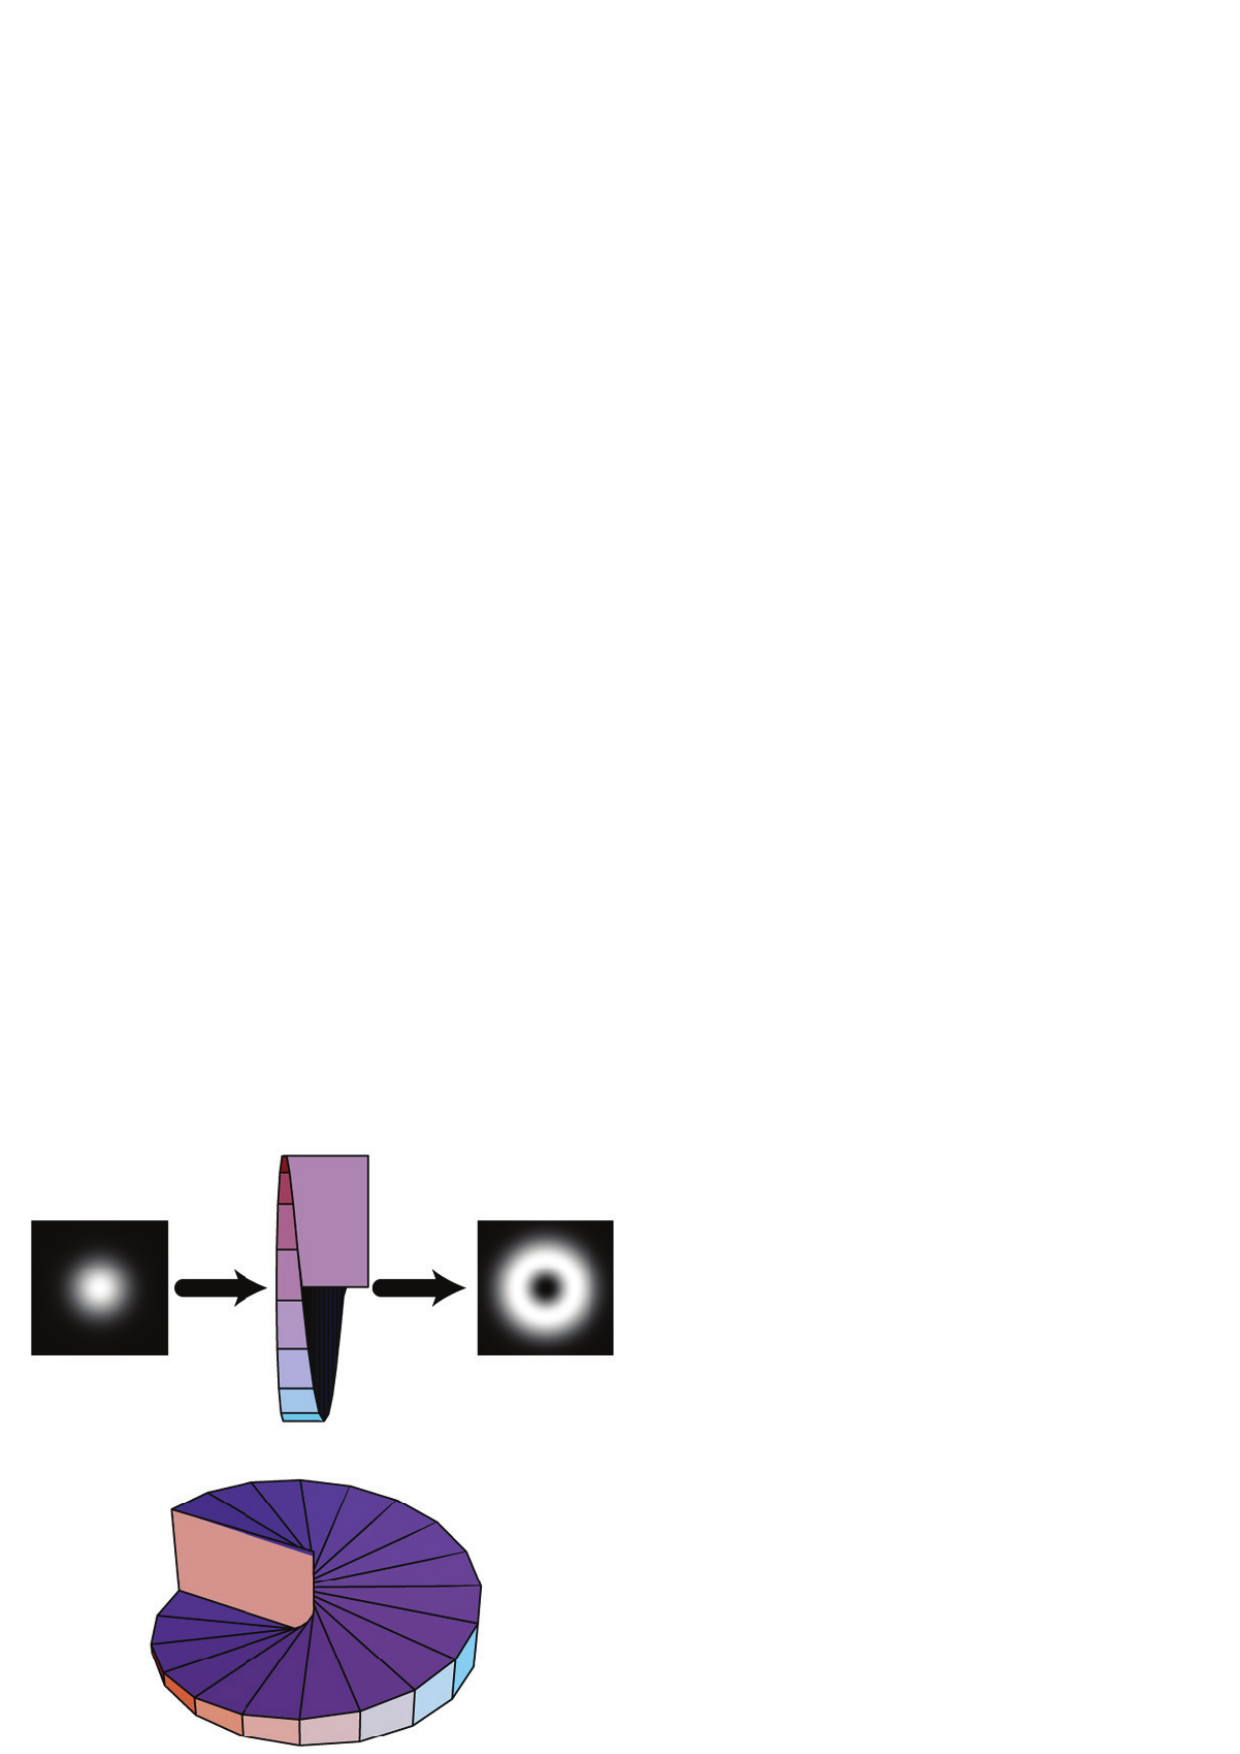
\includegraphics[scale=0.7]{Caps/Imagenes/SPP.png}
  \caption[Placa de fase espiral obtenida por métodos holográficos]{Placa de fase espiral obtenida por métodos holográficos. Imagen adaptada de Ref.[3].}
  \label{fig:sppreal}
\end{figure}

Existe otro método que consiste en la superposición de una red de difracción con una máscara espiral, conocida también como ``redes de difracción bifurcadas'' (\textit{forked grating}) debido a la forma que toma la máscara. El efecto de la adición de una máscara espiral en la red de difracción es la aparición de una transición adicional en la forma de la red, tal como se muestra en la Fig. \ref{fig:forkred}. Los OVs se generan entonces en los ordenes difractados, de forma que si la carga topológica de la máscaras es $q$, el orden $l$ tiene una carga topológica $ql$, es decir, la carga topológica del orden $l = 2$ es $2q$, con $l = 3$ es $3q$ y así sucesivamente \cite{Bazhenov1990, Bekshaev2008, Bekshaev2009}. Una de las mayores ventajas de las redes de difracción es que no necesariamente tienen que ser de fase, se pueden generar OVs empleando redes de amplitud. La Fig. \ref{fig:blazedVO} es un ejemplo de cómo es la distribución de intensidad producido por una red bifurcada del tipo diente de sierra.\\

\begin{figure}[!ht]
  \centering
    \includegraphics[scale=1]{Caps/Imagenes/Gratings.pdf}
  \caption{Obtención de una red de difracción bifurcada.}
  \label{fig:forkred}
\end{figure}

\begin{figure}[!ht]
  \centering
    \includegraphics[scale=0.8]{Caps/Imagenes/DiffGratVO.pdf}
  \caption[Generación de OV a partir de una red de difracción.]{Generación de OV a partir de una red diente de sierra o blazé. Imagen adaptada de Ref.[1].}
  \label{fig:blazedVO}
\end{figure}

Gracias al desarrollo de las pantallas de cristal líquido y de los hologramas generados por computador, la forma más común de generar OVs se ha dado con moduladores espaciales de luz, su funcionamiento será descrito a continuación.

\section{Moduladores espaciales de luz basados en cristal líquido}
\label{sec:slm}

Un modulador espacial de luz (SLM: \textit{spatial light modulator}), es un dispositivo opto-electrónico que como su nombre lo indica, se encarga de modular espacialmente luz y está constituidos por un arreglo de pantallas de cristal líquido (LCDs: \textit{liquid-crystal display}) \cite{Burman2010}. En este contexto \textit{modular} se entiende como variar controladamente las propiedades de la luz, que pueden ser fase o amplitud. Dichos dispositivos emplean la birrefringencia de los cristales líquidos (LCs: \textit{liquid crystal}), de forma tal que mediante un campo eléctrico se rotan los cristales variando así las propiedades de la luz (este concepto se retomará en la sección \ref{subsec:lcdispopt}) \cite{Gennes2007, Cho1998}. Podemos clasificar los SLMs en tres grandes categorías: de fase, de amplitud y aquellos que acoplan ambos efectos. \\

Los SLMs de amplitud son altamente comerciales y permiten variar la intensidad de la luz pixel a pixel en el arreglo de LCDs, es decir, cuando el campo eléctrico es máximo la mayor parte de la luz pasa, cuando es mínimo la luz es absorbida y en los estados intermedios se deja pasar una fracción de la luz, es decir, son de tramitancia variable. Algunos ejemplos de estos son los televisores LCD y los proyectores de vídeo, en estos últimos existe un tipo donde se combinan tres SLMs para generar color con una matriz RGB como se muestra en la Fig. \ref{fig:proyector}.\\

\begin{figure}[!ht]
  \centering
    \includegraphics[width=\textwidth,keepaspectratio]{Caps/Imagenes/Proyector.png}
  \caption[Funcionamiento de un proyector a partir de SLMs.]{Funcionamiento de un proyector a partir de SLMs, variando la intensidad de cada una de las componentes RGB se genera una matriz tal que la imagen generada es a color. Imagen tomada de \small \url{http://www.duiops.net/hifi/cine-en-casa-pantalla-proyectores-lcd.html}}
  \label{fig:proyector}
\end{figure}

Los SLMs de fase son menos comerciales y por lo general más costosos, a diferencia de los SLMs de amplitud, la idea de este tipo de moduladores es que sean capaces de generar una diferencia de fase entre dos puntos cualquiera del arreglo de LCDs y que no generen cambios en la amplitud, la diferencia de fase debe comprender un rango de al menos $[0 - 2\pi]$, de forma que cualquier variación de fase pueda ser representada, dependiendo la longitud de onda. El desarrollo de estos dispositivos ha propiciado el crecimiento de diversas áreas, entre ellas, holografía digital \cite{Jesacher2008}, donde se emplean como generadores de los objetos a registrar,  y en telecomunicaciones \cite{Ahderom2002} por ejemplo, en donde gracias a que las propiedades de la luz puede modificarse punto a punto, es posible transferir diferente información simultáneamente. La Fig. \ref{fig:slm} muestra un SLM PLUTO-VIS-006-A, el cual es de reflexión y solo de fase. \\

\begin{figure}[!ht]
  \centering
    \includegraphics[scale=0.5]{Caps/Imagenes/SLM.jpg}
  \caption{Modulador espacial de luz HOLOEYE-Pluto.}
  \label{fig:slm}
\end{figure}

%Ahora bien, debido a las características de los SLM, la modulación de fase o amplitud se ve influida por el estado de polarización tanto de entrada como de salida de la luz \cite{Iemmi2001, Moreno2003} y por tanto si se desea una modulación solamente de fase, es necesario caracterizar los estados de polarización ante los cuales esta es máxima. Para este proyecto nos centraremos en el HOLOEYE-LC2002\footnote{\url{http://holoeye.com/spatial-light-modulators/discontinued-devices/}}, que es un SLM de transmisión del tipo nemático trenzado (este concepto se abordará en la sección \ref{subsec:lcdispopt}) y una de sus características es que modula tanto fase como amplitud de manera acoplada, por tanto requiere de una calibración que permita una modulación cercana\footnote{Si se cubre el rango [0 - $2\pi$] es posible representar cualquier valor de fase.} a los $2\pi$y no hayan variaciones considerables en la intensidad. La calibración de un SLM de transmisión puede realizarse a través de un sistema generador-analizador de estados de polarización, de forma que ante diferentes estados de entrada y salida hay mayor modulación de fase o de amplitud, este aspecto se profundizará en el capítulo \ref{cap:implementacion}.

Ahora bien, debido a las características de los SLM, la modulación de fase o amplitud se ve influida por el estado de polarización tanto de entrada como de salida de la luz \cite{Iemmi2001, Moreno2003} y por tanto si se desea una modulación solamente de fase, es necesario caracterizar los estados de polarización ante los cuales esta es máxima. Para este trabajo nos centraremos en el HOLOEYE-LC2002\footnote{\url{http://holoeye.com/spatial-light-modulators/discontinued-devices/}}, que es un SLM de transmisión y una de sus características es que modula fase y amplitud de manera acoplada, por tanto requiere de una calibración que permita una modulación cercana\footnote{Si se cubre el rango [0 - $2\pi$] es posible representar cualquier valor de fase.} a los $2\pi$ y no hayan variaciones considerables en la tramitancia. La calibración de un SLM de transmisión puede realizarse a través de un sistema generador-analizador de estados de polarización, de forma que ante diferentes estados de polarización a la entrada y salida del SLM, haya una mayor modulación de fase o de amplitud.%, este aspecto se profundizará en el capítulo \ref{cap:implementacion}.

%Anteriormente se mencionó que los SLMs dependen de 

%La calibración de un SLM de transmisión puede realizarse a través de un sistema generador-analizador de estados de polarización, de forma que ante diferentes estados de entrada y salida hay mayor modulación de fase o de amplitud \cite{Iemmi2001, Moreno2003}, este aspecto se profundizará en el capítulo \ref{cap:implementacion}.

%Finalmente, para aplicaciones relaciones con la generación de OVs se debe contar con una curva de caracterización que no es entregada por el fabricante. Es importante mencionar que los fabricantes de SLMs tales como HOLOEYE\footnote{\url{http://holoeye.com/}} o Hamamatsu Photonics\footnote{\url{http://www.hamamatsu.com/us/en/index.html}} no entregan el producto caracterizado, la calibración debe ser llevada a cabo por quien quiera emplearlo. Esta calibración se realiza acorde al tipo de SLM, para el proyecto nos centraremos en el HOLOEYE-LC2002 \footnote{\url{http://holoeye.com/spatial-light-modulators/discontinued-devices/}}. El LC2002 es un SLM de transmisión del tipo nemático trenzado (este concepto será trabajado en la sección \ref{subsec:lcdispopt}) y una de sus características es que modula tanto fase como amplitud de manera acoplada, por ello, lo que se busca en su calibración es encontrar un estado de funcionamiento tal que la modulación de fase sea cercana a los $2\pi$ y no hayan variaciones considerables en la intensidad. La calibración de un SLM de transmisión puede realizarse a través de un sistema generador-analizador de estados de polarización, de forma que ante diferentes estados de entrada y salida hay mayor modulación de fase o de amplitud \cite{Iemmi2001, Moreno2003}, este aspecto se profundizará en el capítulo \ref{cap:implementacion}.

\subsection{Cristales líquidos como dispositivos ópticos}
\label{subsec:lcdispopt}

Un cristal líquido es un estado intermedio de la materia que lo poseen algunos compuesto químicos, los cuales comparten características típicas de los líquidos y otras características típicas de los estados cristalinos. Por parte de los líquidos poseen la propiedad de moverse libremente en cualquier dirección, aunque, la mayor parte de los líquidos exhiben propiedades físicas (por ejemplo, eléctricas y magnéticas) isotrópicas por naturaleza, los LCs por su lado son anisotrópicos. Normalmente tienen forma cilíndrica o elipsoidal, lo que hace que posean un eje de simetría llamado \textit{eje director}  y les da la propiedad de ser  \textit{orientables}. Su comportamiento se ve alterado por la temperatura, de hecho, cuando se incrementa la temperatura las moléculas se orientan en cualquier dirección, dando lugar a un líquido isotrópico como se muestra en la Fig. \ref{fig:LC}(a), a esta temperatura se le denomina punto de aclarado (\textit{clearing point}). El estado más común de los LCs se conoce como nemático (\textit{nematic}), en este, las moléculas se mueven libremente en cualquier dirección, aunque mantienen sus ejes directores en la misma dirección (Fig. \ref{fig:LC}(b)). Ahora bien, si se disminuye la temperatura, algunos compuestos de LC adquieren un orden espacial y las moléculas se organizan por capas bidimensionales, y el movimiento se limita solo a las capas Fig. \ref{fig:LC}(c) \cite{Uribe2011}.\\

%En condiciones apropiadas las moléculas de LC poseen un orden de orientación tal que los ejes directores se alinean en la misma dirección, conocido como estado nemático (\textit{nematic}), como se muestra en la Fig. \ref{fig:LC}b. En esta fase, las moléculas del cristal pueden moverse pero no pierden su orientación. Si además de tener un comportamiento nemático, las moléculas poseen un orden, es decir, se organizan por capas como se muestra en la Fig. \ref{fig:LC}c se dice que están en estado esméctico (\textit{smectic}) y el movimiento de las moléculas se da solo por capas \cite{Uribe2011}.

\begin{figure}[!ht]
  \centering
    \includegraphics[width=12cm,keepaspectratio]{Caps/Imagenes/LC.pdf}
  \caption[Estados del cristal líquido.]{Estados del cristal líquido. ((a) líquido isotrópico, (b) nemático y (c) esméctico).}
  \label{fig:LC}
\end{figure}

Una consecuencia de la anisotropía de las moléculas, que proviene de la diferencia de la movilidad de los electrones en las dirección longitudinal y transversal al interior del cristal, es poseer distintas propiedades ópticas y eléctricas en diferentes direcciones si consideramos una onda propagándose en dirección paralela o perpendicular al eje director. Este efecto genera dos fenómenos interesantes, la birrefringencia de las moléculas y la orientación bajo la influencia de un campo eléctrico \cite{Uribe2011, Burman2010}. Dada la diferencia entre la movilidad de los electrones al interior del cristal, un campo eléctrico experimenta dos permitividades o constantes dieléctricas distintas, esto se conoce como anisotropía dieléctrica y produce que el desplazamiento eléctrico y el momento dipolar inducido no necesariamente sea paralelo al campo, como consecuencia, los cristales sufren un torque sobre su eje director de forma tal que éste se alinea con la dirección del campo. Una representación de esto puede observarse en la Fig. \ref{fig:torqueLC}, en ausencia de capo eléctrico, la molécula tiene una orientación vertical Fig. \ref{fig:torqueLC}(a), cuando un campo eléctrico representado por las flechas rojas actúa sobre una molécula de LC ésta experimenta un torque (representado por las flechas verdes) causado por la anisotropía Fig. \ref{fig:torqueLC}(b) y la molécula tiende a rotar su eje director en la dirección del campo. Por último si el campo es lo suficientemente intenso, la molécula rota hasta alinearse completamente con la dirección del campo Fig. \ref{fig:torqueLC}(c). \\

\begin{figure}[!ht]
  \centering
    \includegraphics[width=\textwidth,keepaspectratio]{Caps/Imagenes/torqueLC.pdf}
  \caption[Molécula de LC sometida a un campo eléctrico]{Molécula de LC sometida a un campo eléctrico.((a) Torque ejercido a la molécula cuando se aplica un campo eléctrico; (b) con la presencia del campo, la molécula rota para alienar su eje director con la dirección del campo; (c) si el campo es lo suficientemente intenso, el eje director se alinea con la dirección del campo).}
  \label{fig:torqueLC}
\end{figure}

%La forma más común de encontrar los LCs son las LCDs y allí hay una categoría muy común que son los LCDs de  tipo nemático trenzado (TN-LCD: \textit{twisted-nematic liquid-crystal display}).

Una de las configuraciones más comunes para los LCs son las pantallas de cristal líquido (LCD: \textit{liquid-crystal display}). Las LCDs se encuentran en un configuración común conocida como pantallas de cristal líquido \textit{twisted nematic} (TN-LCD: \textit{twisted-nematic liquid-crystal display}). En este, el cristal líquido se encierra entre dos placas de polímero pulido en una dirección específica, llamadas placas de alineación, de forma que el eje director de los cristales se alinea en dirección paralela al sentido del pulido, es decir, hay una prealineación de las moléculas. Las placas son pulidas en direcciones perpendiculares, de forma tal, que las moléculas en contacto con el polímero están en direcciones perpendiculares. Como estamos en el estado nemático, las moléculas de LC tienden a alinear sus ejes directores y a causa de la perpendicularidad entre las moléculas en la superficie del polímero se da un efecto de giro en los ejes directores de las partículas en el interior de la celda, como se muestra en la Fig. \ref{fig:lcd}. Detrás del polímero se ubican dos placas conductoras  transparentes, comúnmente de oxido de indio y estaño (ITO: \textit{indium tin oxide}), de forma que es posible aplicar una diferencia de potencial y por tanto un campo eléctrico a los LCs. En presencia del campo eléctrico, como se mencionó anteriormente, los ejes directores tienden a alinearse con la dirección de este y por tanto hay una rotación de las moléculas. En esta rotación, las propiedades del medio se hacen homogéneas puesto que las moléculas se encuentran alineadas \cite{Uribe2011, Burman2010}. Comúnmente en una celda se ubican dos polarizadores, uno en la entrada y otro en la salida, de forma tal que la rotación de las moléculas permite regular cuánta luz pasa a través de la celda mediante la rotación de los estados de polarización. Pero en los laboratorios, es común que los polarizadores se supriman y que se empleen estados de polarización generados por un sistema generador-analizador para someter la LCD a condiciones de modulación de amplitud o fase de acuerdo a la aplicación.

\begin{figure}[!ht]
  \centering
    \includegraphics[width=\textwidth,keepaspectratio]{Caps/Imagenes/lcdcelda.png}
  \caption[Celda de LCD \textit{twisted nematic}]{Celda de LCD \textit{twisted nematic}. Cuando no hay campo eléctrico, las moléculas de LC rotan su eje director en función de la dirección de las placas de alineación y por tanto la polarización de la luz rota y se transmite por el segundo polarizador. Cuando ese aplica un campo eléctrico, las moléculas se alinean en la dirección del campo, no hay cambio en la polarización de la luz por tanto no hay luz transmitida. Imagen adaptada de Ref. [11].}
  \label{fig:lcd}
\end{figure}

%\section{Consecuencias de por los moduladores espaciales de luz en la generación de vórtices ópticos}
\section{Aberraciones en vórtices ópticos}
\label{sec:genvoslm}


Cuando se se emplean SLMs para obtener haces con vorticidad óptica, actuando estos como generadores de fases espirales, la manera más apropiada de hacerlo es presentar un holograma generado por computadora que contenga información de una máscara de fase espiral (SPM: \textit{spiral phase mask}). El problema de esto es que cuando se quiere generar una máscara cuya carga topológica sea $1$, se requiere de un SLM capaz de generar un cambio de fase de al menos $2\pi$ y que este cambio incremente proporcionalmente con el campo eléctrico aplicado. Consideraremos entonces una modulación ideal, a aquella que además de alcanzar un cambio de fase de $2\pi$, posee una relación lineal entre el cambio de fase y el campo eléctrico aplicado al LC. En el caso del LC-2002 a causa de su modulación acoplada, cuando se tienen modulaciones de fase cercanas a $2\pi$ las variaciones en amplitud son considerables y por esto, es necesario emplear menores modulaciones de fase de forma tal que la variación en intensidad sea despreciable. Emplear una menor modulación de fase para representar la SPM implica un cambio de fase indeseado puesto que la máscara no cumple las condiciones óptimas y por tanto, hay una aberración inducida en los OVs, tal como se muestra en la Fig. \ref{fig:voslm}. Cuando la modulación es ideal y el sistema óptico está limitado por difracción (Fig. \ref{fig:voslm}(a)), se pueden generar SPM con modulaciones de $2\pi$ lineales (Fig. \ref{fig:voslm}(b)) y por tanto se generan OVs ideales (Fig. \ref{fig:voslm}(c)), pero por otro lado, cuando la modulación no es ideal así el sistema óptico siga siendo limitado por difracción(Fig. \ref{fig:voslm}(d)), la SPM tienen un perfil diferente (Fig. \ref{fig:voslm}(e)) y por tanto, es de esperar que el OV generado difiera del ideal (Fig. \ref{fig:voslm}(f)), esta deformación da lugar una aberración inducida por el SLM.\\


%Cuando se se emplean SLMs en la generación de OVs como generador de fases espirales, la manera más apropiada de hacerlo es presentar un holograma generado por computadora que contenga información de una máscara de fase espiral (SPM: \textit{spiral phase mask}). El problema de esto es que cuando se quiere generar una máscara cuya carga topológica sea $1$, se requiere de un SLM capaz de modular al menos $2\pi$ en fase y en condiciones ideales con una curva de modulación lineal. En el caso del LC-2002 a causa de su modulación acoplada, cuando se tienen modulaciones de fase cercanas a $2\pi$ las variaciones en amplitud son considerables y por esto, es necesario emplear menores modulaciones de fase de forma tal que la variación en intensidad sea despreciable. Emplear una menor modulación de fase para representar la SPM implica un cambio de fase indeseado puesto que la máscara no cumple las condiciones óptimas y por tanto, hay una aberración inducida en los OVs, tal como se muestra en la Fig. \ref{fig:voslm}. Cuando la modulación es ideal y el sistema óptico está limitado por difracción (Fig. \ref{fig:voslm}(a)), se pueden generar SPM con modulaciones de $2\pi$ lineales (Fig. \ref{fig:voslm}(b)) y por tanto se generan OVs ideales (Fig. \ref{fig:voslm}(c)), pero por otro lado, cuando la modulación no es ideal así el sistema óptico siga siendo limitado por difracción(Fig. \ref{fig:voslm}(d)), la SPM tienen un perfil diferente (Fig. \ref{fig:voslm}e) y por tanto, es de esperar que el OV generado difiera del ideal (Fig. \ref{fig:voslm}(f)), esta deformación puede considerarse una aberración inducida por el SLM.\\

\begin{figure}[!ht]
  \centering
    \includegraphics[width=\textwidth,keepaspectratio]{Caps/Imagenes/ovsimreal.pdf}
  \caption[Simulación de OVs ideales y generados con un LC-2002.]{Simulación de vórtices ópticos ideal y generado con un SLM LC-2002. ((a) Curva de modulación ideal, (b) SPM obtenida con una curva de modulación ideal, (c) OV generado de manera ideal, (d) curva de modulación experimental, (e) SPM creada experimentalmente; (f) OV obtenido con la modulación real).}
  \label{fig:voslm}
\end{figure}

Como es bien sabido, cuando un campo se propaga a través de un sistema óptico este es susceptible a aberraciones que pueden ser producidas por los elementos ópticos, las aberraciones se manifiestan como una perdida en la resolución de la imagen recuperada a partir de un objeto\footnote{Este tema será tratado posteriormente en la sección \ref{sec:aberraciones}}. Conocer las aberraciones permite su corrección mediante la manipulación del sistema óptico, por ejemplo, si conocemos que la aberración de nuestro sistema óptico es a causa de un desalineamiento, este podría ser intervenido experimentalmente a través de la realineación del sistema; o mediante la adición de un desfase que contrarreste el aporte de las aberraciones \cite{Liesener2004, Cizmar2011}. Dentro de los métodos más comunes de recuperación de fase existen dos categorías en las cuales tenemos los métodos interferométricos (directos) y los no interferométricos (indirectos). En el caso de los métodos intereferométricos \cite{Creath1988, Malacara2007}, a partir de un patrón de interferencia puede encontrarse la fase de un campo objeto y las aberraciones del sistema, para esto existen diversos métodos y algoritmos, por ejemplo, el método de 4 pasos, en donde a partir de cuatro intensidades cada una con un salto de fase determinado puede recuperarse la fase inicial; esta fase recuperada puede ser descompuesta en términos de polinomios que represantan aberraciones físicas y una vez conocidas pueden ser compensadas. Por otro lado, los métodos no interferométricos se basan en las medidas de intensidad directamente \cite{Soloviev2006, Chanan2000}. Un ejemplo de esto es el sensor Shack-Hartmann, en el cual a partir de un arreglo de microlentes sensa el el frente de onda a través del calculo de la desviación de los centros focales.\\

A través de la determinación de las aberraciones producidas por los elementos sistema óptico en los OVs, pueden también corregirse las aberraciones que estos presentan. En nuestro caso, proponemos implementar un método de recuperación de fase no interferométrico que se conoce como diversidad de fase, este concepto lo trataremos en el siguiente capítulo.